\documentclass{article}
\usepackage{graphicx}
\usepackage[margin=1.5cm]{geometry}
\usepackage{amsmath}

\begin{document}
\twocolumn

\title{Thursday Warm Up, Unit 0: Foundations and Fundamentals}
\author{Prof. Jordan C. Hanson}
\maketitle

\section{Memory Bank}
\small
\begin{itemize}
\item $\bar{x} = \frac{1}{N}\sum_{i=0}^{N-1} x_i$ ... Sample mean.
\item $\overline{x^2} = \frac{1}{N}\sum_{i=0}^{N-1} x_i^2$ ... Sample mean of the square.
\item $s = \frac{1}{N-1}\sum_{i=0}^{N-1} (x_i - \bar{x})^2$ ... Sample std. deviation.
\item $s^2 = \overline{x^2} - \overline{x}^2$ ... Formula for the variance.
\item Let a \textbf{histogram} be defined by $M$ bins $i$, with the data organized into $M$ \textit{frequencies} $H_i$.
\item Total number of data points in a histogram: $N = \sum_{i=0}^{M-1} H_i$
\item (1) Sample mean and (2) variance from histograms: 
\begin{enumerate}
\item $\bar{x} = \frac{1}{N}\sum_{i=0}^{M-1} i H_i$
\item $s = \frac{1}{N-1}\sum_{i=0}^{M-1} (i-\bar{x})^2 H_i$
\end{enumerate}
\item For the following two formulas: $\omega = 2\pi f$, $\tau = RC$.
\item \textbf{Low-pass filter response}, as a function of frequency:
\begin{equation}
R(f) = \frac{1}{1+j\omega \tau}
\end{equation}
\item \textbf{High-pass filter response}, as a function of frequency:
\begin{equation}
R(f) = \frac{j\omega\tau}{1+j\omega \tau}
\end{equation}
\end{itemize}
\normalsize

\section{Application of Complex Numbers: AC Circuit Filters}

\begin{enumerate}
\item (a) Suppose a signal has an amplitude of $A$ at a frequency $f$: $A(f)$.  The filtered amplitude is $R(f) A(f)$.  If $A=3.3$ at $f = 50$ kHz, $R = 1$ k$\Omega$, and $C = 1$ $\mu$F, what is the filtered amplitude $A(f) R(f)$, if the filter is \textit{low-pass}? (b) Suppose a signal has an amplitude of $A$ at a frequency $f$: $A(f)$.  The filtered amplitude is $R(f) A(f)$.  If $A=3.3$ at $f = 5$ kHz, $R = 100$ k$\Omega$, and $C = 1$ $\mu$F, what is the filtered amplitude $A(f) R(f)$, if the filter is \textit{high-pass}? \\ \vspace{4cm}
\end{enumerate}

\section{ADC and DAC}

\begin{enumerate}
\item Consider Fig. \ref{fig:1}, which is adapted from Ch. 3 of the course text, when completing the following exercises:
\small
\begin{itemize}
\item If the sampling rate is 10 kHz, and the analog signal frequency is 2.5 kHz, what is the sampled frequency? \\ \\
\item If the sampling rate is 10 kHz, and the analog signal frequency is 5 kHz, what is the sampled frequency? \\ \\
\item If the sampling rate is 10 kHz, and the analog signal frequency is 15 kHz, what is the sampled frequency? \\ \\
\item If the sampling rate is 10 kHz, and the analog signal frequency is 20 kHz, what is the sampled frequency? \\ \\
\end{itemize}
\normalsize
\item If an analog signal is created by a DAC with range [0,5] V, and a max count of 4095, what is its amplitude if the DAC value is 2048 counts? \\ \\
\item If a 4.0 V analog signal is created by a DAC with a max count of 4095, and its amplitude is 1024 in DAC counts, what is the maximum voltage range of the DAC if the minimum is 0 V? \\ \\
\end{enumerate}

\begin{figure}[hb]
\centering
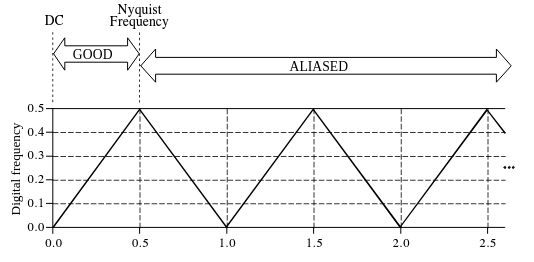
\includegraphics[width=0.5\textwidth]{aliasing.png}
\caption{\label{fig:1} Digital versus analog frequency of sampled signals.}
\end{figure}

\end{document}
